\section{Resultados}
\begin{figure}[H]
  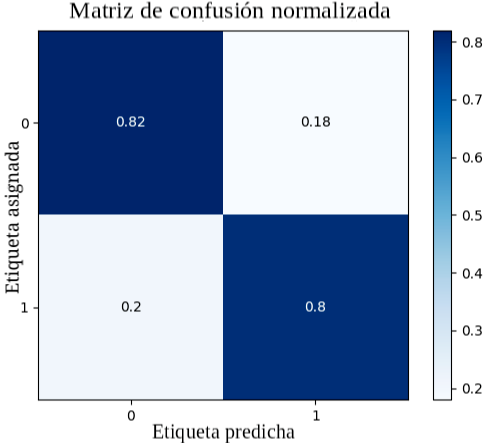
\includegraphics[scale=0.5]{confusion} \centering
  \caption{Matriz de confusión de las predicciones de la red,
  donde la etiqueta 1 representa una pose válida y 0 una inválida.
  Los puntajes son adquiridos a partir del conjunto de validación
  usado durante el entrenamiento, que contiene 2500 poses.}
\end{figure}

\begin{figure}[H]
  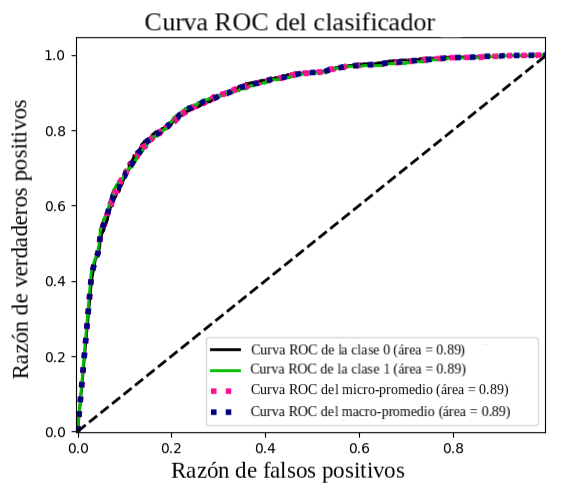
\includegraphics[scale=0.5]{roc_classifier} \centering
  \caption{Curva característica operativa del receptor (ROC,
  \textit{Receptive Operating Characteristic}) mostrando
  las razones de verdaderos y falsos positivos.}
\end{figure}

\begin{figure}[h]
  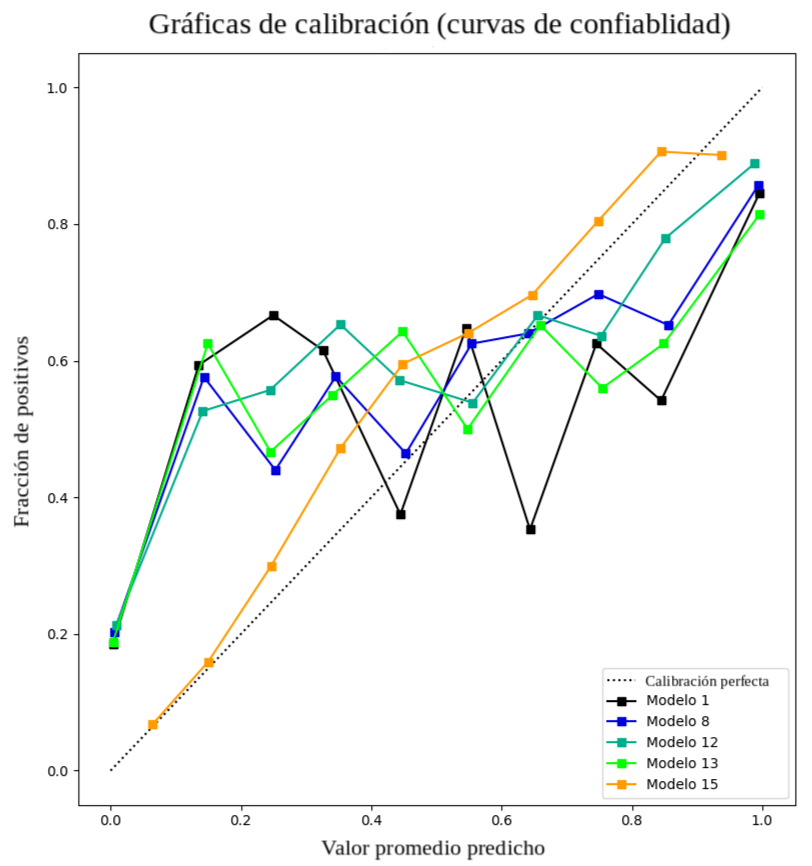
\includegraphics[scale=0.45]{calibration} \centering
  \caption{Calibracion de los hiperparámetros, siendo la iteración
  número 15 la mejor encontrada.}
\end{figure}

En este trabajo se diseña y se crea \textit{Deep-pose}: una red de
aprendizaje profundo que busca hacer ua evaluación de acoplamientos
virtuales. \textit{Deep-pose} está compuesta por una capa
convolucional, una capa oculta y una de clasificación y toma como
entrada la salida de acoplamientso virtuales generados por AutoDock
Vina. Estos acoplamientos son traducidos en una codificación que
transforma las poses de acoplamiento en vectores de enteros mediante
asociaciones con tablas de búsqueda, y sirven como entrada a la red.

Esta arquitectura, permitó obtener un 82\% de precisión al momento de
discernir entre poses cercanas a las cristalográficas. Este resultado,
aunado a que (1) \textit{Deep-pose} no requiere características
definidas por un humano, a diferencia del proceso \textit{artesanal}
que se sigue usualmente para determinar cuáles acoplamientos son
buenos, y que (2) alcanza buenos resultados a partir de la salida de
un sólo programa de docking, hacen que \textit{Deep-pose} sea
atractivo para usarse como complemento al acoplamiento virtual usado
normalmente. Además, este trabajo propone ideas novedosas sobre cómo
modelar complejos proteínas-ligandos e introduce una propuesta que
demuestra ser efectiva para codificar configuraciones moleculares, que
podría ser usada para otros fines en alguna otra red de aprendizaje
profundo aplicada a bioinformática.
